\chapter{Introduction}

\section{Project context}

The Underground Mining Monitoring System (UMMS) is a software-based monitoring application designed to detect and evaluate potentially hazardous environmental conditions in underground mining environments. The system processes sensor data, evaluates safety-related thresholds, and triggers appropriate system responses when abnormal situations are detected.


This document defines the test specification for the software developed in the Advanced Programming project. The goal of the project is to implement a reliable monitoring application that processes sensor data, evaluates system conditions, and reacts to abnormal situations according to defined system requirements. The execution of these tests ensures that the implemented functionality operates reliably and that the system transitions between its operational states as intended.

The software architecture consists of several modular components (see Figure~\ref{fig:umms_overview} below for more context) responsible for tasks such as sensor data processing, filtering, system monitoring, and state management. These components interact within a structured application framework and are executed periodically by the system scheduler.

\begin{figure}[H]
    \centering
    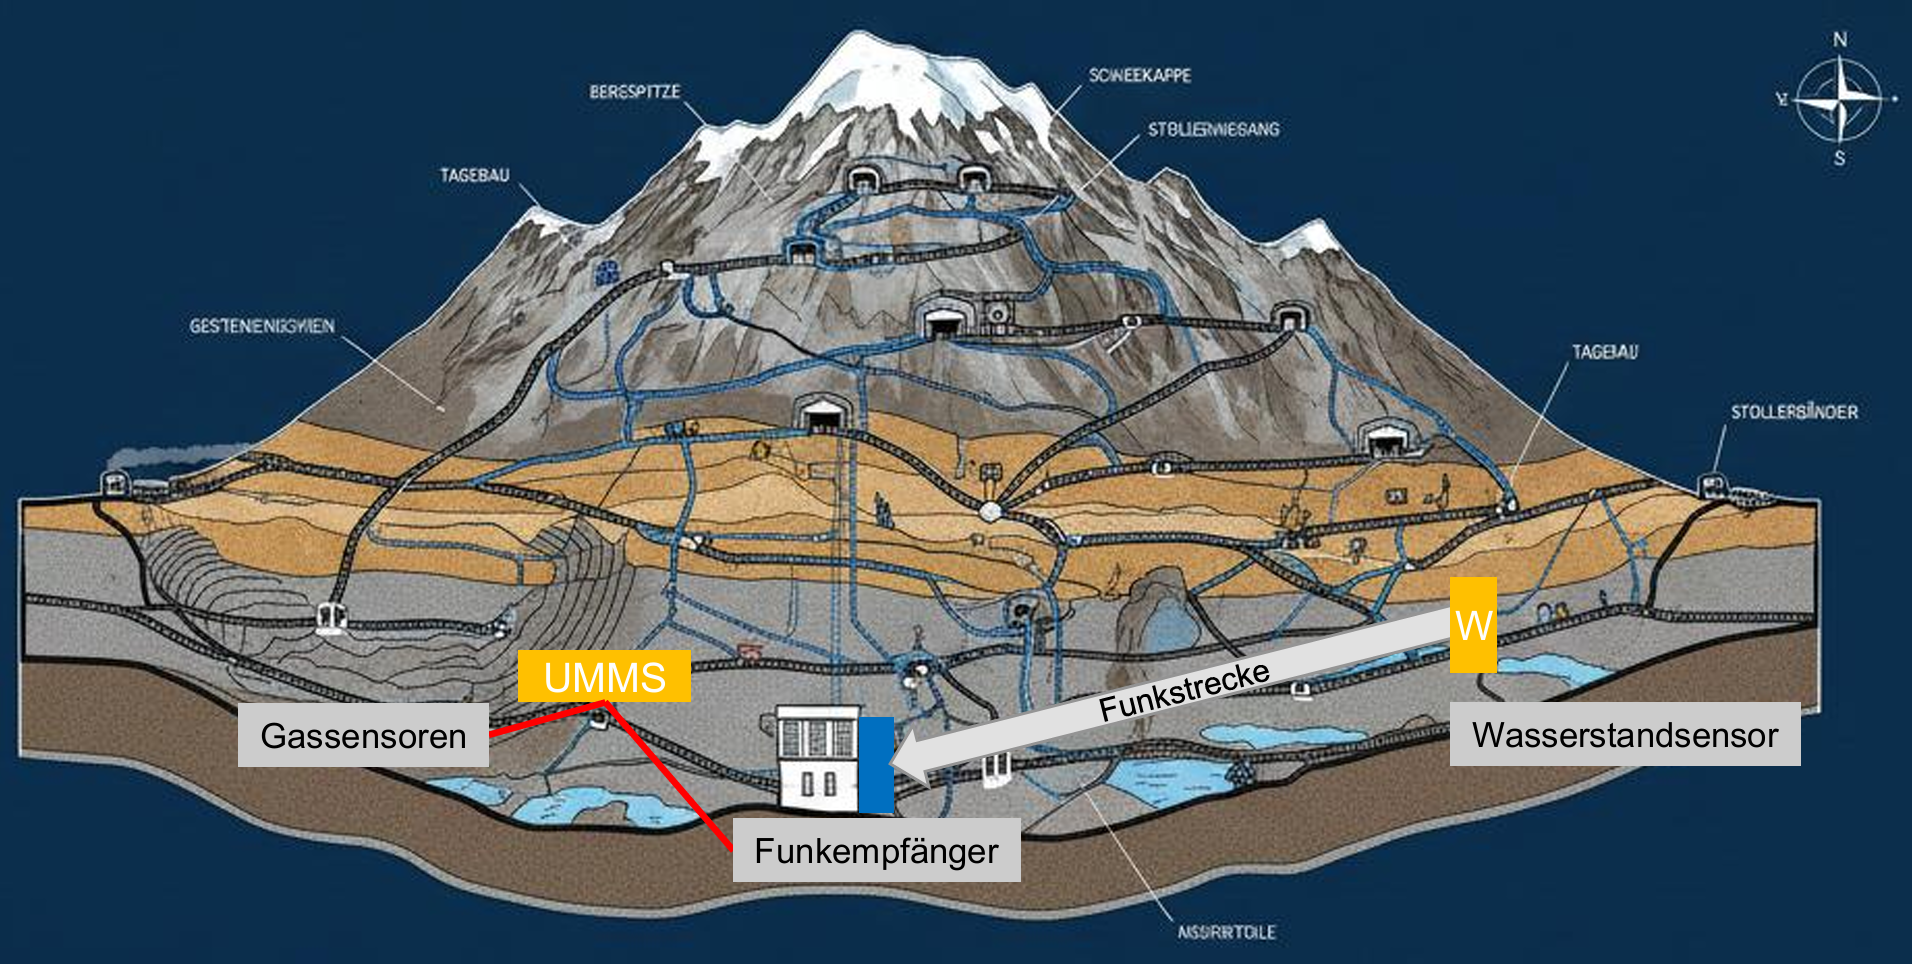
\includegraphics[width=0.85\linewidth]{figures/umms.png}
    \caption{System context of the Underground Mining Monitoring System (UMMS)}
    \label{fig:umms_overview}
\end{figure}

\section{Disclaimer regarding the UART interface towards the water sensor}

During the development of the system, the project requirements regarding the water sensor input were modified. In the current version of the requirements, the water sensor value is provided as a constant value rather than being received via the UART interface. To ensure compliance with the updated specification, the final implementation therefore uses a predefined constant value for the water sensor input within the application logic.

It should be noted, however, that the functionality for receiving and processing water sensor data via UART was already implemented during earlier development stages. This functionality is contained within the \textit{RadioConnect} module, which includes the mechanisms for receiving, buffering, and processing the corresponding serial data. Although this module remains part of the project codebase, its UART-based data reception is currently not invoked by the application due to the revised requirements.